\chapter{Marco Te\'orico}
\section{Palabras Clave}
Las palabras clave se definen como una secuencia de una o mas palabras que idealmente
proveen una representaci\'on compacta de la esencia del contenido de un 
documento. \cite{REC10}
%TODO: Complentar la definici\'on (usos, aplicaciones)

\section {Clasificaci\'on de documentos}
La clasificaci\'on de documentos se refiere al problema de asignar un documento a
uno o m\'as categor\'ias, esta tarea puede ser realizada manualmente, generalmente
por expertos en bibliotecolog\'ia, o de forma automatizada.

\section{Lenguaje Natural}
Es el lenguaje hablado o escrito por humanos para prop\'ositos generales
de comunicaci\'on. Son aquellas lenguas que han sido generadas
espont\'aneamente en un grupo de hablantes con el prop\'osito de
comunicarse, a diferencia de otras lenguajes, como pueden ser un lenguaje
construido, lenguajes de programaci\'on o los lenguajes usados en el
estudio de la l\'ogica formal, especialmente la l\'ogica matem\'atica.

\section{Lexicograf\'ia}
La lexicograf\'ia se define como la \emph{praxis de la lexicolog\'ia} que se ocupa
de la elaboraci\'on de diccionarios \cite{LEX01}. \\

La metalexicograf\'ia estudia aspectos te\'oricos de los diccionarios, tales como
su historia, tipolog\'ia, finalidad y su relaci\'on con otras disciplinas. \\

\section{Procesamiento del Lenguaje Natural}
El Procesamiento del Lenguaje Natural (PLN) es la disciplina encargada
de producir sistemas inform\'aticos que posibiliten la comunicaci\'on
hombre-computadora por medio del lenguaje humano a trav\'ez de la voz o
del texto escrito.

\section{Modelo TextRank}
Es un m\'odelo de puntuaci\'on basado en grafos para el procesamiento de
texto \cite{RMPT04}, que es utilizado para la extracci\'on de palabras claves
y sentencias mediante algoritmos de puntuaci\'on basados en grafos.
% TODO: Completar este concepto

\subsection{Algoritmos de puntuaci\'on basados en grafos}
Son algoritmos que se utilizan para obtener valores significativos
(\emph{calificaci\'on}) de los nodos en un grafo. \\

Existen varios algoritmos de puntuaci\'on: \emph{PageRank} de Google,
\emph{HITS} de Kleinberg, \emph{Positional Function} de Herings \cite{RM04}. \\

A continuaci\'on se describe el algoritmo PageRank.

\subsubsection{Algoritmo PageRank}
\begin{figure}
	\centering
		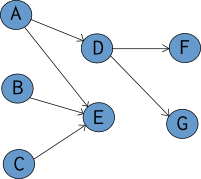
\includegraphics[]{recursos/img/grafoDirigido}
		\caption {Grafo dirigido}
\end{figure}

Dado $G=(V,E)$ un grafo dirigido, con un conjunto de v\'ertices $V$ y un conjunto
de arcos $E$, donde $E$ es un subconjunto de $V x V$, llamamos $In(V_i)$ al
conjunto de v\'ertices que apuntan a $V_i$ (predecesores),  en la Figura 2.1
$In(E)=\{A,B,C\}$, y $Out(V_i)$ al conjunto de v\'ertices que son apuntados por $(V_i)$
(sucesores), en la Figura 2.1 $Out(D)=\{F,G\}$ . El puntaje del v\'ertice $V_i$ 
esta dado por \cite{SBLP98}:

\begin{equation}
	S(V_i) = (1 - d) + d * \sum_{V_j\in In(V_i)}{\frac{1}{|Out(V_j)|}S(V_j)}
\end{equation}

donde $d$ es un factor de amortiguaci\'on que toma valores comprendidos entre
0 y 1, que expresa la probabilidad de avanzar de un v\'ertice a otro de manera
aleatoria, generalmente tiene el valor de 0.85 \cite{SBLP98}.

\subsection{Aplicaci\'on en la extracci\'on de palabras claves}
El grafo es construido de la siguiente manera: se seleccionan palabras  para 
conformar los v\'ertices, si existe una relaci\'on de \emph{co-ocurrencia} entre 
las palabras seleccionadas, se a\~nade un nodo entre ellas. \\

Las palabras seleccionadas son aquellas que pasan por un filtro sint\'actico, el cual
selecciona solo las unidades l\'exicas pertenecientes a un conjunto definido de tipos
de palabras. \\

Se pueden seleccionar todos los tipos de palabras, o un conjunto restringido a verbos
y sustantivos, se presentan mejores resultados con el conjunto de verbos y
adjetivos \cite{RMPT04} .
